\chapter{连续介质力学} \label{chap2}
\section{引言}
连续介质力学是本文构建控制方程的理论基础。
基于连续介质力学,我们刻画流体以及流体表面,并从两个
视角来描述物体运动,以此构建动力学方程。为了构建完整的控制方程,我们还需要给出本构模型,
即形变与应力的关系,这里我们给出对应的流体的弱可压缩模型以及表面张力模型。

\section{欧拉视角下的动力学}
欧拉视角,即物理量的定义域为$\mathbb{R}^3$,对物体的刻画由空间中的密度场给出。与拉格朗日视角的区别我们将在2.3小节中给出。

\subsection{欧拉视角下的质量守恒定律}
记$\rho : \mathbb{R}^3 \times \mathbb{R} \rightarrow \mathbb{R}$ 为空间中随时间变化的密度场,
$v : \mathbb{R}^3 \times \mathbb{R} \rightarrow \mathbb{R}^3$ 为空间中随时间变化的速度场,此处默认向量为列向量。
\begin{figure}[htbp]
    \centering
    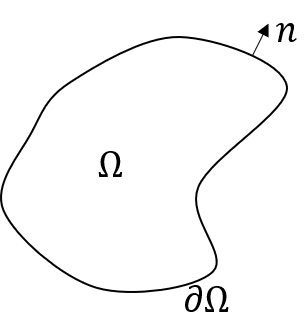
\includegraphics[scale=0.5]{./images/image1.png}
    \caption{区域符号示例}
    \label{fig:domain}
\end{figure}

现在考虑一个闭区域$\Omega$,$\Omega$的边界记为$\partial \Omega$,边界上的外法向记为
$n$,同时假定$\rho$ 和 $v$在 $\Omega$的一个开邻域内足够光滑。根据质量守恒,我们有$\Omega$上质量的
变化率为$\partial \Omega$上质量的流出率和流入率之和。即
\begin{equation}
    \begin{split}
        \frac{d}{dt}\int_{\Omega} \rho(x,t)dx &= -\int_{\partial \Omega} \rho v \cdot n ds \\
        \int_{\Omega} \frac{\partial}{\partial t} \rho (x,t)dx &= -\int_{\partial \Omega} div(\rho v)dx\nonumber\\
    \end{split}
\end{equation}
如果$\rho$在$\mathbb{R}^3$上都能达到足够光滑,那么由$\Omega$的任意性,可知
\begin{equation}
    \frac{\partial}{\partial t}\rho (x,t) + div(\rho v) = 0
\end{equation}

\subsection{欧拉视角下的动量守恒定律}
现在考虑闭区域$\Omega$上的动量变化。根据连续介质力学中的牛顿运动定律[**],闭区域$\Omega$上的动量变化可以分为三部分,
第一部分为物质流入流出$\Omega$导致的动量变化,第二部分为作用在$\Omega$边界上的力导致的动量变化,第三部分为作用在$\Omega$内部物质上的力(一般为重力)产生的作用变化。
即
\begin{equation}
    \frac{d}{dt} \Big |_{t = t_0} \int_{\Omega} \rho v dx = -\int_{\partial \Omega} \rho v (v\cdot n) ds + \int_{\partial \Omega} \sigma \cdot n ds + \int_{\Omega} \rho g dx
\end{equation}
在(2.2)式中,$g$为重力加速度,$\sigma$为Cauthy应力[**]。特别的,$\sigma$是一个三阶对称矩阵,其对称性来源于角动量守恒[**],我们将在2.4节中从另一个角度说明其对称性。

由于(2.2)式中$\Omega$选择的任意性,我们有
\begin{equation}
    \frac{\partial}{\partial t} \Big |_{t = t_0}(\rho v) = -div(\rho v^{T}v) + div(\sigma) + \rho g
\end{equation}

矩阵函数散度$div$定义如下:
\begin{equation}
    \begin{split}
        div &: C^1(\mathbb{R}^3;\mathbb{R}^{3\times 3}) \rightarrow C^1(\mathbb{R}^3;\mathbb{R}^3)\\
        &div(A)_i := \sum_j \partial_j A_{ij}\nonumber\\
    \end{split}
\end{equation}

(2.2)式变形为
\begin{equation}
    \frac{\partial}{\partial t} \Big |_{t = t_0}(\rho v) + div(\rho v^{T}v) = div(\sigma) + \rho g
\end{equation}


\section{拉格朗日视角下的动力学}
在上一节中,我们根据质量守恒和动量守恒得到了两个方程(方程(2.1)与方程(2.4)),非常重要的一点是,上述方程并没有使用任何
有关自然状态--材料在不施加外力的静止状态--的信息。在之后的章节中,我们将假定,$t=0$是处于自然状态,并且只考虑$t \ge 0$ 的情况。

假定在自然状态下($t = 0$),材料占据的空间为$\Omega_0 \subset \mathbb{R}^3$,此时也称$\Omega_0$为参考构型。对于任意给定的$t\in (0,+\infty)$,
此时材料占据的空间为$\Omega_t \subset \mathbb{R}^3$,相对于参考构型$\Omega_0$,称$\Omega_t$为当前构型。

拉格朗日视角和欧拉视角的区别主要是函数的定义域。在上一节中,我们所有函数的定义域都在$\mathbb{R}^3$上,而本节我们将把视角限制在材料上,例如对于任意时刻$t$,
有$\Omega_t$上的实值函数,$f(\cdot,t) :\Omega_t \rightarrow \mathbb{R} $。

\subsection{形变映射,形变梯度,速度}
为了描述材料相对于参考构型发生的形变,我们引入形变映射 $$\phi:\Omega_0 \times [0,+\infty) \rightarrow \mathbb{R}^3$$,形变映射同时也给出了物体的运动轨迹。
为了方便,我们记$\phi_t (x) = \phi(x,t)$,实际上我们还假定$\{ \phi_t(x): t\in \mathbb{R}\}$构成了一个单参数变换群,并且关于$t$至少二阶光滑,关于$X$至少有连续的一阶导数。

有了形变映射,我们可以引入对局部形变的刻画,即形变梯度$F(X,t):=\frac{\partial \phi_t(X)}{\partial X}$。实际上,形变梯度$F(X,t)$还可以视为$X$处切空间的映射,即
$$F(X,t):T_X \Omega_0 \rightarrow T_x \Omega_t$$
对于任意的$\partial_X \in T_X \Omega_0$, $\partial_x = F(X,t)[\partial_X] \in \Omega_t$,
即形变梯度将$X$点的切向量$\partial_X$经过平移起始点,旋转方向,拉伸长度后得到$x$点的切向量$\partial_x$,如图2.2所示。
\begin{figure}[htbp]
    \centering
    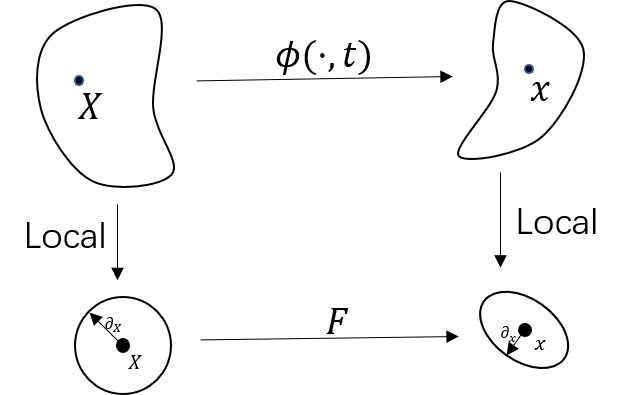
\includegraphics[scale=1.0]{./images/image2.png}
    \caption{形变与形变梯度}
    \label{fig:deformation gradient}
\end{figure}

同样的,形变映射作为单参数变换群,自然的导出速度的定义$V(X,t):= \frac{\partial \phi_t(X)}{\partial t}$。 值得注意的是,$V(X,t)$的定义域是在$\Omega_0$上,其值域
是一个起始点在$\Omega_t$上的一个三维列向量,其与欧拉视角下定义的速度关系为$V(X,t) = v(\phi_t(X),t)$,如果记$x = \phi_t(X)$,则$V(X,t) = v(x,t)$。

考察$F$关于时间的一阶导
\begin{equation}
    \begin{split}
        \frac{d}{dt}F(X,t) &= \frac{d}{dt}\frac{\partial}{\partial X}\phi_t\\
        &= \frac{\partial}{\partial X} \frac{d}{dt} \phi_t\\
        &= \frac{\partial}{\partial X} V(X,t)\\
        &= \frac{\partial v(\phi_t(X),t)}{\partial x}\frac{\partial \phi_t}{\partial X}\\
        &= \frac{\partial v(x,t)}{\partial x}\frac{\partial \phi_t}{\partial X}\\
        &= \nabla v \cdot F\nonumber
    \end{split}
\end{equation}
整理后我们得到$F$和$v$的关系
\begin{equation}
    \dot{F} = \nabla v \cdot F
\end{equation}


\subsection{拉格朗日视角下的质量守恒}
在引入了形变$\phi_t$之后,很自然的有$\hat{\Omega}_t = \{\phi_t(X):X\in \hat{\Omega}_0 \subset \Omega_0 \}$(简记为$\phi_t(\hat{\Omega}_0)$),且$\hat{\Omega}_t \subset \Omega_t$,
根据质量守恒,形变不会影响质量,即
$$\int_{\hat{\Omega}_0} \rho(x,0)dx = \int_{\hat{\Omega}_t} \rho(x,t)dx = \int_{\phi_t(\hat{\Omega}_0)} \rho(x,t)dx$$
如果我们将$\hat{\Omega}_t$的质量记为$M[\hat{\Omega}_t]$,则有$\frac{d}{dt}M[\hat{\Omega}_t] = 0$。而
\begin{equation}
    \begin{split}
        \frac{d}{dt} \int_{\phi_t(\hat{\Omega}_0)} \rho(x,t)dx &= \frac{d}{dt} \int_{\hat{\Omega}_0} \rho(\phi_t(X),t) det(F(X,t))dX\\
        &= \int_{\hat{\Omega}_0} \frac{d}{dt} [\rho(\phi_t(X),t) det(F(X,t))] dX \\
        &= 0\nonumber
    \end{split}
\end{equation}

记 $R(X,t):=\rho(\phi_t(X),t)$,$J(X,t):=det(F(X,t))$, 则根据$\hat{\Omega}_0$的任意性,有$\frac{d}{dt}[R(X,t)J(X,t)] = 0$,即
\begin{equation}
    R(X,t)J(X,t) = R(X,0)
\end{equation}
(2.6)式即为拉格朗日视角下的质量守恒方程。
\subsection{拉格朗日视角下的动量守恒}
在拉格朗日视角下,$\hat{\Omega}_{0}$的动量变化可以表示为作用在$\hat{\Omega}_{0}$边界上的力以及作用在$\hat{\Omega}_{0}$
内部的力之和。即
\begin{equation}
    \begin{split}
        \frac{d}{dt}\Big |_{t = t_0}\int_{\hat{\Omega}_0}R(X,0)V(x,t)dX = \int_{\partial \hat{\Omega}_{0}} P \cdot N dS + \int_{\hat{\Omega}_{0}} R(X,0) g dX
    \end{split}
\end{equation}
上式实际上对于任意的$\hat{\Omega}_0$成立,因此有以下
\begin{equation}
    R(X,0)\frac{\partial}{\partial t} V(X,t) = DIV(P) + Rg
\end{equation}
此处$DIV$是$\Omega_0$上的散度算子,为了与$\Omega_t$上进行区分记为大写。其中$P$是应力的另一种表述形式,称为First Piola–Kirchhoff应力[**],其满足$\int_{\partial \hat{\Omega}_{0}} P \cdot N dS = \int_{\partial \hat{\Omega}_{t}} \sigma \cdot n ds$
我们将在下一节本构关系中更详细的给出$P$的计算方式以及与$\sigma$的关系。 

下面我们再次从拉格朗日视角推导欧拉视角下的动量守恒,来证明两者的等价性。
\begin{equation}
    \begin{split}
        \frac{d}{dt}\Big |_{t = t_0}\int_{\hat{\Omega}_0}R(X,0)V(x,t)dX &= \frac{d}{dt}\Big |_{t = t_0} \int_{\hat{\Omega}_0}R(X,t)v(\phi_t(X),t)J(X,t)dX\\
        &=\int_{\hat{\Omega}_0} \frac{d}{dt}\Big |_{t = t_0} [\rho(\phi_t(X),t)v(\phi_t(X),t)J(X,t)]dX\\
        &=\int_{\hat{\Omega}_0} \frac{d}{dt}\Big |_{t = t_0} [\rho(\phi_t(X),t)v(\phi_t(X),t)J(X,t)]dX\\
        &=\int_{\hat{\Omega}_0} v(\phi_{t_0}(X),t_0)\frac{d}{dt}\Big |_{t = t_0}[\rho(\phi_t(X),t) J(X,t)] \\
        &+ \rho(\phi_{t_0}(X),{t_0})J(X,t_0)\frac{d}{dt}\Big |_{t = t_0} v(\phi_{t_0}(X),t_0) dX\nonumber\\
        &=\int_{\hat{\Omega}_0}v(\phi_{t_0}(X),t_0)\frac{d}{dt}\Big |_{t = t_0}R(X,0) \\
        &+ \rho(\phi_{t_0}(X),{t_0})J(X,t_0)\frac{d}{dt}\Big |_{t = t_0} v(\phi_{t}(X),t)dX\\
        &=\int_{\hat{\Omega}_0}\rho(\phi_{t_0}(X),{t_0})J(X,t_0)\frac{d}{dt}\Big |_{t = t_0} v(\phi_{t}(X),t)dX\\
        &=\int_{\hat{\Omega}_{t_0}}\rho(x,t_0)\frac{d}{dt}\Big |_{t = t_0} v(\phi_{t,t_0}(x),t)dx\nonumber
    \end{split}
\end{equation}
这里$\phi_{t,t_0} = \phi_t \cdot \phi_{t_0}^{-1}$,带入(2.6)中就有
\begin{equation}
    \begin{split}
        \int_{\hat{\Omega}_{t_0}}\rho(x,t_0)\frac{d}{dt}\Big |_{t = t_0} v(\phi_{t,t_0}(x),t)dx = \int_{\hat{\Omega}_{t_0}} div(\sigma) dx + \int_{\hat{\Omega}_{t_0}} \rho g dx\nonumber
    \end{split}
\end{equation}
这里由于$\hat{\Omega}_{t_0}$为$\Omega_t$内的任意闭区域,因此
$$\rho(x,t_0)\frac{d}{dt}\Big |_{t = t_0} v(\phi_{t,t_0}(x),t) = div(\sigma) + \rho g$$

其中$$\frac{d}{dt}\Big |_{t = t_0} v(\phi_{t,t_0}(x),t) = \frac{\partial}{\partial t}\Big |_{t = t_0}v(x,t) + \sum_i \frac{\partial \phi_{t,t_0}^i}{\partial t}  \cdot \frac{\partial}{\partial x_i}v(x,t_0) = \frac{\partial}{\partial t}\Big |_{t = t_0}v(x,t) + v^T\nabla v$$
这里$\phi_{t,t_0}^i$为$\phi_{t,t_0}$的第$i$个分量。
此处引入材料时间导数$\frac{D}{Dt}f := \frac{\partial}{\partial t} f + v\nabla f $,将其代入上式中整理得
\begin{equation}
    \begin{split}
        \rho \frac{Dv}{Dt} = div(\sigma) + \rho g
    \end{split}
\end{equation}
该方程实际与(2.4)式等价,由于其更简洁的表述形式,我们之后将称(2.9)式为欧拉视角下的动量守恒。
$$\frac{\partial}{\partial t}(\rho v) + div(\rho v^{T}v) = div(\sigma) + \rho g$$
可考察方程的左端项
\begin{align*}
    \frac{\partial}{\partial t}(\rho v) + div(\rho v^{T}v) & = \rho \frac{\partial}{\partial t} v + v \frac{\partial}{\partial t} \rho + \rho v^T\nabla v + v div(\rho v)                           \\
                                                           & = \rho (\frac{\partial}{\partial t} v + v^T\nabla v) + v(\frac{\partial}{\partial t} \rho + div(\rho v))     & \text{第二项为质量守恒} \\
                                                           & = \rho \frac{Dv}{Dt}
\end{align*}
带入即知,(2.4)式是(2.8)式的展开。

\section{本构关系}
在前两节中,我们在动量守恒方程中引入了应力项,其决定了速度如何随着时间变化。本节我们将给出如何通过形变来给出
应变张量,其中应变张量和形变的函数关系被称为本构关系。事实上,本构关系直接决定了我们模拟的物体会表现出何种特质。

流体被认为是一种不可压缩的物质,用数学的语言就是说其形变梯度$F$满足$det(F)\equiv 1$,然而在实践中,为了更好的配合物质点法的使用,
我们从要求$det(F)\equiv 1$转变为使用形变能量密度来惩罚形变对体积的影响,$W(F):= \frac{\lambda}{2} (det(F) - 1)^2$。可以发现,对任意的$F\in \mathbb{R}^{3\times 3}, U\in SO_3$,始终有$W(UF) = W(F)$,
该特性被称为旋转不变性,根据诺特定理[**],如果能量密度是旋转不变的,那么所得到的系统是角动量守恒的。

在有了能量密度函数,我们推导能量密度变化量和形变梯度的变化量之间的关系
\begin{equation}
    \begin{split}
        \delta W(F)&= \frac{\lambda}{2}\delta (det(F) - 1)^2\\
        &= \lambda (det(F) - 1) \delta(det(F) - 1)\\
        &= \lambda (det(F) - 1) \delta(det(F)) \nonumber\\
    \end{split}
\end{equation}
为了计算$\delta det(F)$,首先考察$\frac{d}{dt}\Big |_{t = 0}det(F + tI)$,由矩阵的特征多项式得
$$det(F + \epsilon I) = \epsilon ^n + \epsilon ^{n-1}Tr(F) + ... + det(F)$$
则等式两边同时除$\epsilon^n$得
$$det(\frac{1}{\epsilon}F + I) = 1 + \frac{1}{\epsilon} * Tr(F) + ... + \frac{1}{\epsilon^n} det(F)$$
此时将$t\neq 0$代入有
$$det(tF + I) = 1 + t Tr(F) + ... + t^ndet(F)$$
同时验证$t=0$可知上式恒成立。
因此$\frac{d}{dt}\Big |_{t = 0}det(tF + I) = tr(F)$,
现在对于任意的$t_0$以及$\mathbb{R}^{3 \times 3}$中通过$A(t_0)$(假设$A(t_0)$可逆)的一条光滑路径$A(t)$,我们有对应的通过$I$的路径
$A(t_0)^{-1}A(t)$,其对应的切向量为$A(t_0)^{-1}\frac{d}{dt}\Big |_{t=t_0}A(t)$,则
\begin{equation}
    \begin{split}
        \frac{d}{dt}\Big |_{t = t_0} det(A(t)) &= \lim_{h \to 0} \frac{det(A(t_0 + h)) - det(A(t_0))}{h}\\
        &=det(A(t)) \lim_{h\to 0} \frac{det(A(t_0)^{-1}A(t_0 + h)) -1}{h}\\
        &= det(A(t))tr(A(t_0)^{-1}\frac{d}{dt}\Big |_{t=t_0}A(t))\\
        &= det(A(t))A(t_0)^{-T}:\frac{d}{dt}\Big |_{t=t_0}A(t)
    \end{split}
\end{equation}
这里$A:B:=\sum_{i,j}A_{ij}B_{ij}$。

故$\delta det(F) = det(F) F^{-T}:\delta F$,代入$\delta W(F)$之中即有$$\delta W(F) = \lambda (det(F) - 1)det(F) F^{-T}:\delta F$$
,其中$P = \lambda (det(F) - 1)det(F)F^{-T}$被称为First Piola–Kirchhoff应力,其与Cauthy应力$\sigma$的关系[**]为
$$J\sigma = PF^{T}$$
我们将在本小节最后给出该关系式的证明,代入可知柯西应力$\sigma = \lambda (det(F) - 1)I$。

这里的$W(F)$实际上只给出了物体的抗压缩性的性质,我们还需要给出表面张力的能量密度函数。根据[**],表面能实际和物体表面积成正比,表面张力为表面能的梯度。那么我们首先可以
形变和表面能量的关系
\begin{equation}
    S(\phi_t) = k\int_{\phi_t (\partial \Omega_0)} ds
\end{equation}
为了更好的计算其梯度,我们对(2.10)式做一些处理。此处引入一些微分流形的记号[**],记$f^*$为$f$导出的拉回映射,$f_*$为推前映射,$ds,d\tilde{s}$分别为曲面$\partial \Omega_{t_0}, \partial \Omega_{t}$上的面积二形式,其为空间体积形式$dv$内乘法向的结果,
即$ds(X,Y) = dv(n,X,Y)$,我们记$ds = dv\odot n$,$ \tilde{p} = \phi_{t_0,t}(p)$,则对任意的$t \in[0, t_0),\tilde{X},\tilde{Y}\in T_{\tilde{p}}\Omega_t$有如下
\begin{equation}
    \begin{split}
        (\phi_{t_0,t}^*ds) (\tilde{X},\tilde{Y})& = (\phi_{t_0,t}^* (dv \odot n))(\tilde{X},\tilde{Y})\\
        &= ((\phi_{t_0,t}^* dv)\odot(\phi_{t_0,t}^* n))(\tilde{X},\tilde{Y})\\
        &= det(F(x;t_0,t))dv (<F^{-1}(x;t_0,t)n,\tilde{n}>\tilde{n} ,\tilde{X},\tilde{Y})\\
        &= det(F(x;t_0,t))<F^{-1}(x;t_0,t)n,\tilde{n}> dv(\tilde{n} ,\tilde{X},\tilde{Y})\\
        &= det(F(x;t_0,t))<n,F^{-T}(x;t_0,t)\tilde{n}>dv(\tilde{n} ,\tilde{X},\tilde{Y})
    \end{split}
\end{equation}
上式中$F(x;t_0,t) = \frac{\partial \phi_{t_0,t}(x)}{\partial x}$,$\tilde{n}$为$T_{\tilde{p}}\Omega_t$单位法向,$<\cdot,\cdot>$为空间内积,容易验证$F^{-T}(x;t_0,t)\tilde{n}$与$T_p\Omega_0$垂直,
故$<n,F^{-T}(x;t_0,t)\tilde{n}> = \Vert F^{-T}(x;t_0,t)\tilde{n}\Vert$, 即$\Vert F^{-T}(x;t_0,t)\tilde{n}\Vert n = F^{-T}(x;t_0,t)\tilde{n}$,那么有
$$(\phi_{t_0,t}^*ds) = det(F(x;t_0,t)) \Vert F^{-T}(x;t_0,t)\tilde{n}\Vert d\tilde{s}$$
则代入表面能表达式有
\begin{equation}
    \begin{split}
        S(\phi_{t_0}) &= k  \int_{\partial\Omega_{t_0}}ds\\
        &= k \int_{\phi_{t_0,t}(\partial\Omega_{t})} ds\\
        &= k \int_{\partial \Omega_t}  \phi_{t_0,t}^* ds\\
        &= k \int_{\partial \Omega_t} det(F(x;t_0,t)) \Vert F^{-T}(x;t_0,t)\tilde{n}\Vert d\tilde{s}\nonumber\\
    \end{split}
\end{equation}

至此,我们得到表面能的另一个表达形式
\begin{equation}
    \begin{split}
        S(\phi_{t_0}) = k \int_{\partial \Omega_t} det(F(x;t_0,t)) \Vert F^{-T}(x;t_0,t)\tilde{n}\Vert d\tilde{s}
    \end{split}
\end{equation}
(2.21)式将是表面张力离散化的基础。

最后,我们给出$J\sigma = PF^{T}$的证明,
\begin{align*}
    \int_{\partial \hat{\Omega}_{t}} \sigma \cdot n ds &= \int_{\phi_t (\partial \hat{\Omega}_{0})} \sigma\cdot n ds\\
    &= \int_{\partial \hat{\Omega}_0} \phi_t^*(\sigma\cdot n) (\phi_t^* ds)\\
    &= \int_{\partial \hat{\Omega}_0} \sigma\cdot n J \Vert F^{-T} N\Vert dS\\
    &= \int_{\partial \hat{\Omega}_0} \sigma F^{-T} \cdot F^{T}n J \Vert F^{-T} N\Vert dS\\
    &= \int_{\partial \hat{\Omega}_0} J\Vert F^{-T} N\Vert\sigma F^{-T} \cdot \frac{1}{\Vert F^{-T}N \Vert} N dS\\
    &= \int_{\partial \hat{\Omega}_0} J\sigma F^{-T} \cdot N dS\\
\end{align*}
而$\int_{\partial \hat{\Omega}_{0}} P \cdot N dS = \int_{\partial \hat{\Omega}_{t}} \sigma \cdot n ds$,因此$\int_{\partial \hat{\Omega}_0} J\sigma F^{-T} \cdot N dS = \int_{\partial \hat{\Omega}_0} P \cdot N dS$,
由于上式对任意$\partial \hat{\Omega}_0$成立,则$J\sigma F^{-T}= P$得$J\sigma = PF^{T}$。


\section{本章小结}
本章基于连续介质力学得到了一系列的控制方程
\begin{align*}
    &\frac{\partial}{\partial t}\rho (x,t) + div(\rho v) = 0 & \text{欧拉视角下的质量守恒方程} \\
    &R(X,t)J(X,t) = R(X,0) & \text{拉格朗日视角下的质量守恒方程} \\
    &\rho \frac{Dv}{Dt} = div(\sigma) + \rho g & \text{欧拉视角下的动量守恒方程}\\
    &R(X,0)\frac{\partial}{\partial t} V(X,t) = DIV(P) + Rg &\text{拉格朗日视角下的质量守恒方程}
\end{align*}

以上四个方程分别从两种视角分别等价的刻画了质量守恒和动量守恒,这两种视角也会在物质点法离散化的过程中体现出来。其次,我们还给出了
形变梯度与速度的关系
\begin{align*}
    \dot{F} = \nabla v \cdot F
\end{align*}
该方程将会在物质点法如何获得下一时刻的形变梯度中起到关键作用。最后,
我们给出了弱可压缩能量$W(F)=\lambda (J-1)^2$来刻画流体的特性,该能量也给出了First Piola–Kirchhoff应力和Cauthy应力的计算方式。
其次我们给出了表面能的计算方法
$$S(\phi_{t_0}) = k \int_{\partial \Omega_{t_1}} det(F(x;t_0,t_1)) \Vert F^{-T}(x;t_0,t_1)\tilde{n}\Vert d\tilde{s}$$
该计算形式下,积分域不随着$\phi_{t_0}$变化而变化,为我们离散计算以及变分都带来了便利,而表面张力将由表面能变分获得,这一步我们将在离散化的过程中来计算。







